\subsection{Wrist Modulation - FiLM}\todo{wwaaffle more coherently, relate to depsep}
The results here are following the proposed modulation 6 wrist RGB and depth modulation techniques from Section \ref{subsec:policies-film}. Each variant of this policy has some hyperparameters associated with it. I landed on using the following after preliminary testing reasoning and about the structure of the data.

For \textbf{LATE} models, with the initial learnt down-sampling and the FiLM module
\begin{itemize}
  \item Initial Downsampling Network, which does $3$ convolutions takes in a \(\langle 3, ~64, ~64 \rangle\) image and returns features of shape \(\langle 16, ~4, ~4 \rangle \)
  \item Then the FiLM module takes in two of these feature vectors and does the modulation. The resulting encoding size is \(16 \times 4 \times 4 = 256\) as FiLM does change the shape of the given tensor.
  \item If there is bi-modulation the final encoding is double the size, $512$, as the modulated vectors are concatenated.
\end{itemize}

For \textbf{NON-LATE} models:
\begin{itemize}
  \item Shallow encoder, used to match the channel dimension of modalities, is a single \verb|Conv2d|  that upsamples the channel dimensions to $6$ while preserving width and height ($64 \times 64$), \todo[color=green]{again appendix}.
  \item The FiLM network as before does not change the sizes returns \(\langle 12, ~64, ~64 \rangle \) or \(\langle 6, ~64, ~64 \rangle \) respectively if it is bi-modulation or not.
  \item Finally there is another CNN that encodes these modulated features, see \todo[color=green]{appendix}, which have layers $\left[36, ~72, ~128, ~128\right]$ and $\left[32, ~48, ~64, ~128\right]$ respectively to bi or not. The final feature size is \(\langle 128, ~2, ~2 \rangle\) regardless.
\end{itemize}
The grasp variants of these were trained over \(\left[ 100, ~200, ~400, ~600, ~800\right]\) epochs, after identifying the grasp task does not benefit from training for too long.


\subsubsection{Grasp - Normal}
The baseline's line (in blue) is also included in the final distance graph for easy comparison. Immediate observations from, Figure \ref{fig:film-grasp-final}, is that any modulation, reaches the similar final distances both the wrist and the wrist and depth data was reaching beforehand in the baseline. Early modulation seems to be more effective in understanding the `control' task so learning the trained distribution, however late modulation not only more successful at grasping the target Figure \ref{fig:film-grasp-success}, but also reaches closer to the `test' sample. 

Success of early modulation is also higher than the baseline \ref{subfig:base-grasp-control-success-smaller}. However, the `test' grasping is no better. Even though the late modulated version have some chance and that is better than the baseline, the puny 1-2\% could be attributed to random chance \todo[color=red]{compare the grasp attempts of these, if there are more grasp attempts but failures it is not random chance but better learning of wwhen to grasp, but the mvement is bad (late does not reach asclose, so maybe grasping is good, but do a table of grasp attempts versus successful grasps??)}

\begin{figure}[H]
  \centering
  
\includegraphics[width=\linewidth]{assets/evaluation/film/film-grasp-final.png}
  \caption{Final Distances Reached for the Grasp task \textbf{normal}}\label{fig:film-grasp-final}
\end{figure}\todo[color=red]{include the baseline wrist rbg+depth line in this graph}

\begin{figure}[H]
  \centering
  \begin{subfigure}{0.45\linewidth}
    \centering
    \includegraphics[width=\linewidth]{assets/evaluation/film/film-grasp-success.png}
    \caption{Grasp success per epoch and over seeds for `Control' and `Test'}\label{subfig:film-grasp-success}
  \end{subfigure}
  \hfill
  \begin{subfigure}{0.45\linewidth}
    \centering
    \includegraphics[width=\linewidth]{assets/evaluation/film/film-grasp-control-success-epochs.png}
    \caption{Success for `Control' per Epoch (shared legend)}\label{subfig:film-grasp-control-success-epoochs}
  \end{subfigure}
  
  \caption{Grasp Success for the FiLMed configurations}\label{fig:film-grasp-success2}
\end{figure}\todo{tabify this list}

\subsection{Grasp - Smaller}
We finally have a module that seems to improve its success rate \ref{fig:film-grasp-success}. While the distance distribution still seems to be similar to the baseline \ref{fig:film-grasp-final-smaller}. This is probably because when the task is not successful the arm will move around a bit more and potentially move slightly away. The 10cm is still within the grippers view range, the wrist camera i mounted around 8cm form the gripper tip. Although the `test' (now \textbf{normal}) is more better the `control' is not benefiting from this \ref{subfig:film-grasp-control-success-epoochs}. I think this is only  due to the smaller target being tougher to grab. if the gripper does not fully align with the target the grasp is almost always unsuccessful. \todo{include some grasping pictures here??}


\begin{figure}[H]
  \centering
  
\includegraphics[width=\linewidth]{assets/evaluation/film/film-grasp-final-smaller.png}
  \caption{Final Distances Reached for the Grasp task \textbf{smaller}}\label{fig:film-grasp-final-smaller}
\end{figure}\todo[color=red]{include the baseline wrist rbg+depth line in this graph}

\begin{figure}[H]
  \centering
  \begin{subfigure}{0.30\linewidth}
    \centering
    \includegraphics[width=\linewidth]{assets/evaluation/film/film-grasp-success-smaller.png}
    \caption{Grasp success per epoch for `Control' and `Test'}\label{subfig:film-smaller-grasp-success}
  \end{subfigure}
  \hfill
  \begin{subfigure}{0.30\linewidth}
    \centering
    \includegraphics[width=\linewidth]{assets/evaluation/film/film-grasp-control-success-epochs-smaller.png}
    \caption{Success for `Control' per Epoch (shared legend)}\label{subfig:film-grasp-control-success-epochs}
  \end{subfigure}
  \hfill
  \begin{subfigure}{0.30\linewidth}
    \centering
    \includegraphics[width=\linewidth]{assets/evaluation/film/film-grasp-test-success-epochs-smaller.png}
    \caption{Success for `Test' per Epoch (shared legend)}\label{subfig:film-grasp-test-success-epoochs}
  \end{subfigure}
  
  \caption{Grasp Success for the FiLMed configurations}\label{fig:film-grasp-success}
\end{figure}


\subsubsection{Reach Results}
The heightened depth understanding capabilities are also seen here \ref{fig:film-reach}. The minimum distances reached by the FiLM policies are all below the obstacle and closer than the baseline. In the grasping task, double modulation seems to perform better. However, in the reaching task ``Colour modulated Depth'' variants (\verb|W_Dfilm{_LATE}|) are clearly more successful.\todo{why is this?}

\begin{figure}[htpb]
  \centering
  \begin{subfigure}{0.40\linewidth}
    \centering
    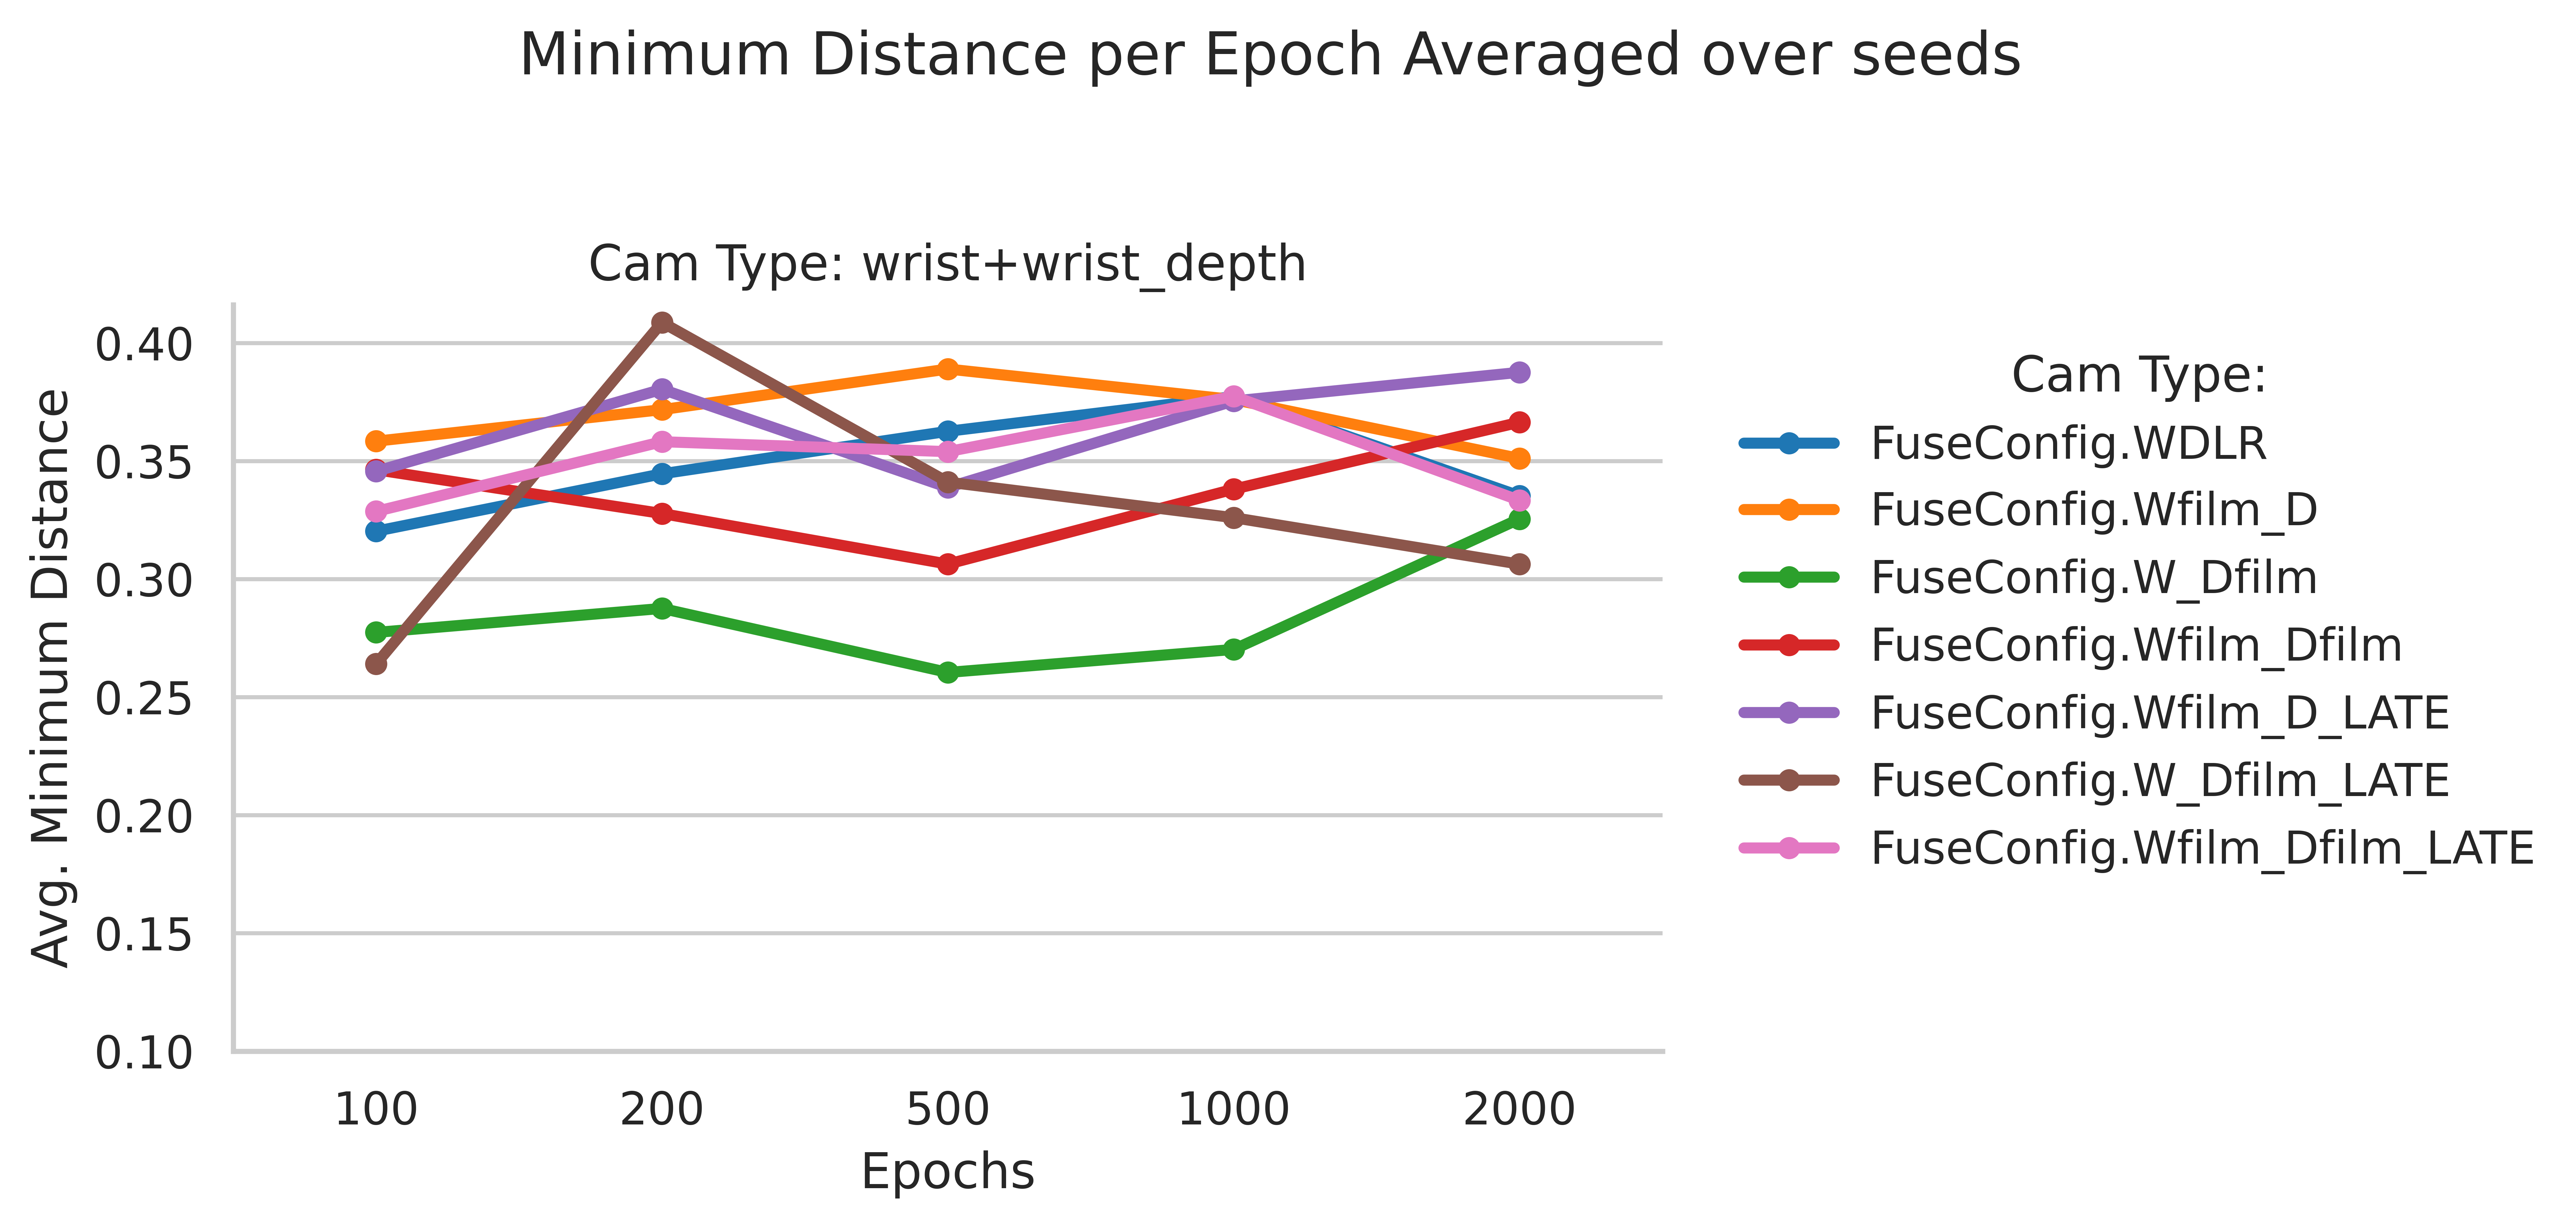
\includegraphics[width=\linewidth]{assets/evaluation/film/reach-min-cams.png}
    \caption{Minimum Distance tor reach target}\label{subfig:film-reach-min}
  \end{subfigure}
  \begin{subfigure}{0.40\linewidth}
    \centering
    \includegraphics[width=\linewidth]{assets/evaluation/film/base-reach-success-config-epochs.png}
    \caption{Reach Success Rates per Epoch}\label{subfig:film-reach-success}
  \end{subfigure}
  \caption{Reach Results}\label{fig:film-reach}
\end{figure}

